\documentclass[12pt,letterpaper,titlepage]{article}

\usepackage{fontspec}
\defaultfontfeatures{Mapping=tex-text}
\usepackage{xunicode}
\usepackage{xltxtra}
\usepackage{amsmath}
\usepackage{pdfpages}
\usepackage{amsfonts}
\usepackage{bbold}
\usepackage{amssymb}
\setcounter{secnumdepth}{0}
\usepackage{nameref}
\usepackage{enumitem}
\usepackage{environ}
\usepackage{pgfplots}
\usepackage{listings}

\showboxdepth=\maxdimen
\showboxbreadth=\maxdimen


\usepackage{paracol}
\usepackage{wrapfig}
\globalcounter{table}
\globalcounter{figure}
\usepackage{graphicx}
\usepackage[left=1in,right=1in,top=1in,bottom=1in]{geometry}
\graphicspath{{img/}}

\author{Jacob Abel}
\title{	Design \& Simulate 13
	\\\large ECE2204 CRN:82929
}

\setlength{\parskip}{0.5em}

\begin{document}
\maketitle
\begin{raggedright}

\section{Problem 15.3-8.a.1: } 
\subsection{Design}

Modify the circuit below to replace the current source with a resistor $R_S$ and preserve the quiescent point. Design $W/L$ and $R_D$ to bias $I_d = 250\mu A$ and $V_S = -2.25V$. Let $k_n^\prime$ vary by $\pm 5\%$. Compare the stabilities of the Q-points of the two bias schemes (current source vs. resistive) by comparing the $\%$ variations of $I_{dQ}$, $V_{dsQ}$, and $V_{gsQ}$. Assume $V_T = 0.8V$, $k_n^\prime = 80\mu A/V^2$, $V_G = 0$

\begin{center}
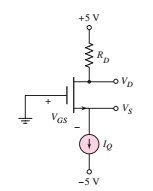
\includegraphics[width=\textwidth, height=12\baselineskip, keepaspectratio=true]{ds1}
\end{center}

\begin{align*}
   V_{GS} 
   	&= V_G - V_S
     = 0V + 2.25V
     = 2.25V
\\ I_D 
	&= \frac{k_n^\prime}{2}\times\frac{W}{L}(V_{GS} - V_{TN})^2
\\ \frac{W}{L} 
    &= \frac{2 I_D}{k_n^\prime(V_{GS} - V_{TN})^2}
	 = \frac{2 (250\mu A)}{(80\mu A/V^2)(2.25V - 0.8V)^2}
	 = 2.97
\\ V_{R_D} 
    &= \frac{V_{DD} - V_{S}}{2}
     = \frac{5 + 2.25V}{2}
     = 3.625V
\\ R_D 
	&= \frac{V_{R_D}}{I_D}
	 = \frac{3.625V}{250\mu A}
	 = 14.5k\Omega
\\ V_{R_S}
	&= V_S - V_{SS}
	 = -2.25V + 5V
	 = 2.75V
\\ R_S
	&= \frac{V_{R_S}}{I_D}
	 = \frac{2.75V}{250\mu A}
	 = 11k\Omega
\end{align*}

Evaluating Modes
\begin{align*}
   k_n^\prime &= [76, 80, 84]\mu A/V^2
\\ V_{DG}
	&= V_T
	 = 0.8V
\\ V_D 
    &= V_G + V_{DG} 
     = 0 + 0.8V = 0.8V
\\ I_D 
	&= \frac{5V-0.8V}{14.5k\Omega} 
 	 = 289.7\mu A
\\ V_{R_S} 
	&= R_SI_D
	 = (11k\Omega)(289.7\mu A)
	 = 3.1867V
\\ V_S
	&= V_{SS} + V_{R_S}
	 = -5V + 3.1867V
	 = -1.813V
\\ V_{GS}
	&= V_G - V_S
	 = 0 + 1.813V
	 = 1.813V
\\ V_{GS}^\prime
	&= \sqrt{\frac{2I_D}{K_n^\prime}\frac{W}{L}} + |V_T|
	 = \sqrt{\frac{2(289.7\mu A)}{[76, 80, 84]\mu A/V^2(2.97)}} + |0.8V|
	 = [2.402, 2.362, 2.324]V
\\ 
\end{align*}

As all $V_{GS}^\prime > V_{GS}$, the transistor is in saturation mode.

\begin{align*}
   V_{DS}
	&= V_{DD} - V_{SS} - I_D(R_D + R_S)
	 = 5V + 5V - I_D(14.5k\Omega + 11k\Omega)
	 = 10V - I_D(25.5k\Omega)
\\ V_{GS}
	&= V_G - I_DR_S
	 = -I_D(11k\Omega)
\\ I_D
	&= \frac{K_n^\prime W}{2L}(V_{GS} - V_T)
\\  &= \frac{K_n^\prime}{2}(2.97)(-I_D(11k\Omega) - 0.8V)(10V - I_D(25.5k\Omega))^2
\\ I_D(76\mu A/V^2)
	&= 402\mu A
\\ I_D(80\mu A/V^2)
	&= 412\mu A
\\ I_D(84\mu A/V^2)
	&= 420\mu A
\\ V_{DS}(402\mu A)
	&= 10V - (402\mu A)(25.5k\Omega)
\end{align*}

\clearpage
\subsection{Validation}

\begin{center}
LTSpice Implementation (values within $<1\%$)

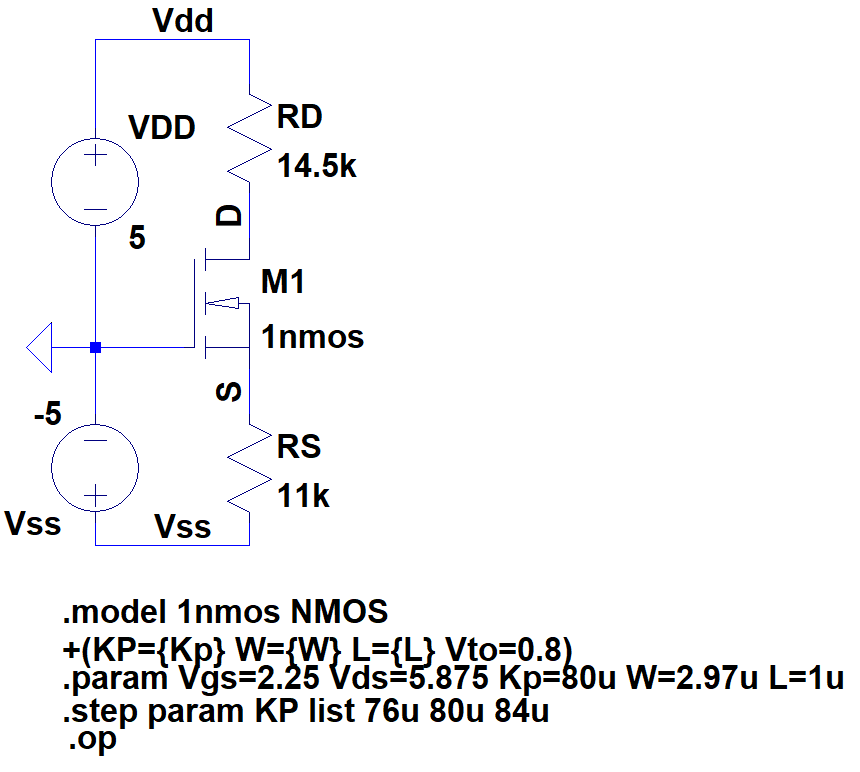
\includegraphics[width=.5\textwidth, height=\textheight, keepaspectratio=true]{ds1b}
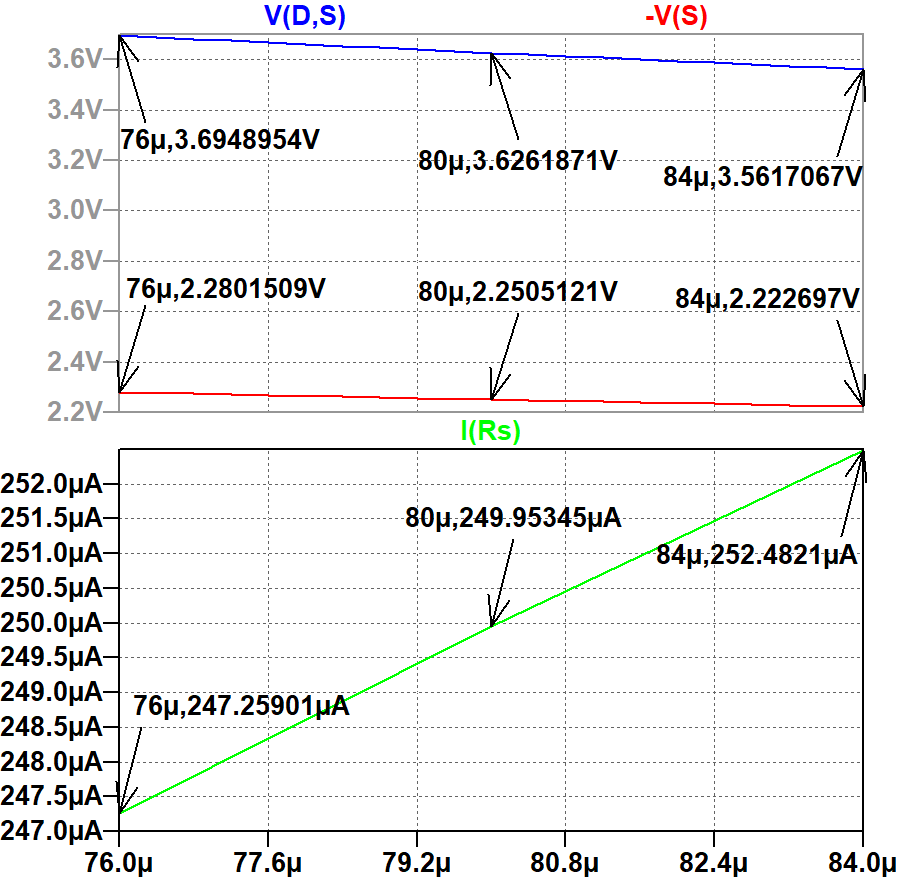
\includegraphics[width=.48\textwidth, height=\textheight, keepaspectratio=true]{ds1c}
\end{center}

I messed something up with this and have been fighting with it for days to no avail. I apologise for submitting this largely incomplete assignment so late.

This assignment should demonstrate a basic understanding of DC analysis of basic MOSFET circuits.

\textit{I have neither given nor received unauthorized assistance on this assignment.}


\end{raggedright}
\end{document}
